\chapter{Conceptos sobre Protocolos}
\label{protocolos}
\section{Definici'on}
Un protocolo de comunicaci'on es un conjunto de reglas y normas de transmisi'on, que permite a dos o m'as entidades, comunicarse entre s'i.

\begin{quote}
\textit{''Un protocolo define el formato y el orden de los mensajes intercambiados entre dos o m'as entidades que se comunican, as'i como las acciones que se toman en la transmisi'on y/o recepci'on de un mensaje u otro evento \citep{redesComputadores}.''}
\end{quote}

Es necesario que, antes de establecer una comunicaci'on entre partes, se definan ciertos protocolos para poder asegurar la interoperabilidad y hacer posible la comunicaci'on entre el emisor y receptor.

Las reglas definen la forma en la que debe efectuarse la comunicaci'on, incluyendo cuestiones como la temporizaci'on, secuencia, revisi'on y correcci'on de errores. Define una \textit{sintaxis} (formato de los mensajes), una \textit{sem'antica} (significado de los mensajes) y \textit{sincronizaci'on} (secuenciamiento y temporizaci'on en la comunicaci'on).

\clearpage

Las tareas a realizar se dividen en niveles (capas), luego, los protocolos de cada capa son los que resuelven las tareas. Definir los modelos en capas brinda las siguientes ventajas:

\begin{enumerate}
\item Dividir la comunicaci'on  en partes m'as peque'nas y sencillas
\item Normalizar los componentes de red para permitir el desarrollo y el soporte de los productos de diferentes fabricantes.
\item Permitir la interoperabilidad de diferentes tipos de hardware y software de red para comunicarse entre s'i.
\item Impedir que los cambios en una capa puedan afectar a las otras capas. Facilita la actualizaci'on del protocolo pudiendo modificar un m'odulo a reemplazarlo todo por completo.
\end{enumerate}

\section{Modelo OSI}
\label{osi}
En los inicios de Internet, hubo un gran crecimiento tanto en cantidad como en tama�o de las redes. Debido a esto, muchas de las redes eran incompatibles entre s'i, y era extremadamente complicada la comunicaci'on entre ellas. Para solucionar este problema, la ISO\footnote{International Standard Organization}, realiz'o ciertas investigaciones acerca de los esquemas de red. En 1980 \citep{zim80}, cre'o un modelo de red para ayudar a los dise�adores de redes a poder implementar redes que puedan comunicarse entre s'i y trabajar en conjunto. Este es el modelo de referencia OSI, definida en la ISO/IEC 7498-1 \citep{osi74981}. Este modelo se agrupa en capas, cada capa agrupa una funci'on determinada. Est'an organizadas jer'arquicamente, cada capa ofrece un servicio a la capa superior. Es un modelo te'orico, toma la experiencia de la pila de protocolos TCP/IP (ver \ref{tcpip}), modelo que soporta Internet.

\clearpage

El modelo tiene 7 capas:
\begin{itemize}
\item[7.] Aplicaci'on
\item[6.] Presentaci'on
\item[5.] Sesi'on
\item[4.] Transporte
\item[3.] Red
\item[2.] Enlace
\item[1.] F'isico
\end{itemize}
Se puede ver su distribuci'on en la Figura \ref{capasOSI}

\begin{figure}[ht!]
  	\centering
	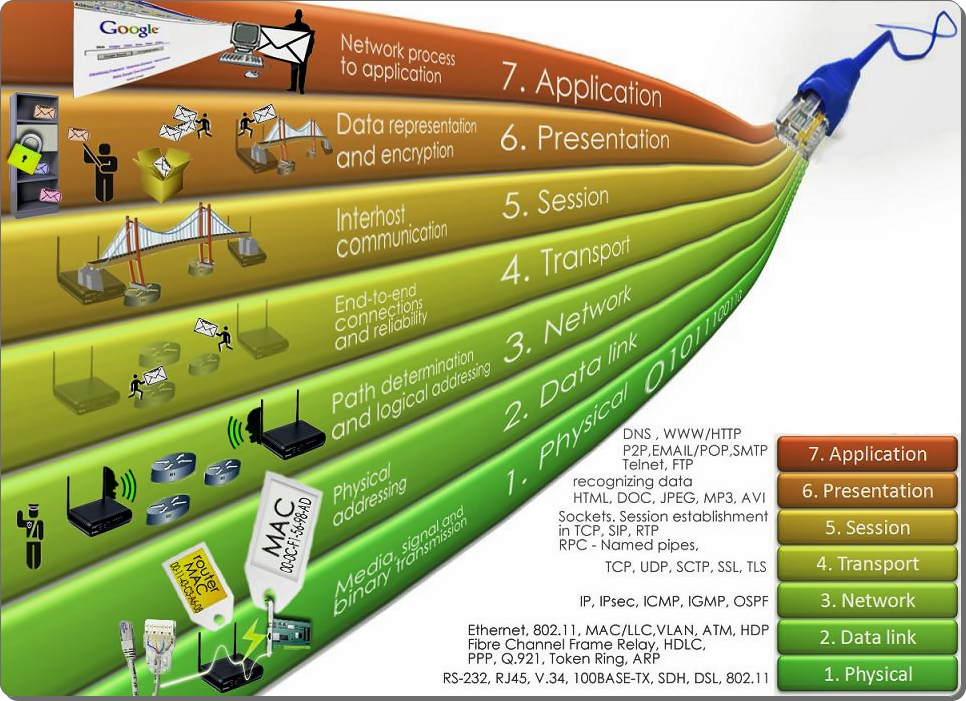
\includegraphics[width=420px]{img/osi}
	\caption{\small Capas OSI, extra'ido de http://www.gargasz.info/}
	\label{capasOSI}
\end{figure}

\clearpage

\subsection{Capa de Aplicaci'on}

Proporciona servicios de red a las aplicaciones del usuario, es la 'unica capa que no provee servicios a otra capa. Si bien es la interfaz hacia el usuario, este no interact'ua directamente con esta capa, sino que lo hace a trav'es de una aplicaci'on que si tiene acceso directo a esta capa.

\subsection{Capa de Presentaci'on}

Define el formato de los datos que se van a intercambiar entre las aplicaciones y ofrece a los programas de aplicaci'on un conjunto de servicios de transformaci'on de datos. Esta capa es la encargada de manejar las estructuras de datos abstractas y realizar las conversiones de representaci'on de datos necesarias para la correcta interpretaci'on de los mismos.

\subsection{Capa de Sesi'on}

Esta capa establece, administra y finaliza las sesiones entre las partes intervinientes en la comunicaci'on, a esto se le llama Servicio de Administraci'on de la Sesi'on. Tambi'en realiza el control del intercambio de datos y sincroniza el di'alogo entre las partes, a esto se le llama Servicio de Administraci'on del Di'alogo.

\subsection{Capa de Transporte}

Esta capa provee un servicio de transporte universal. Ofrece transparencia en el intercambio de datos entre los hosts involucrados (extremo a extremo) y a'isla a las capas superiores de los detalles de implementaci'on del transporte. Asegura que los datos enviados lleguen en el mismo orden en el que han sido enviados y sin errores, brindando calidad de servicio y confiabilidad en la comunicaci'on.

\subsection{Capa de Red}

Se encarga de la conexi'on de hosts que pueden encontrarse en redes diferentes, define un esquema de direccionamiento, enrutamiento y selecci'on de rutas. Permite que los datos viajen de un extremo a otro a trav'es de redes interconectadas. Se utilizan los paquetes como unidad de informaci'on, estos paquetes son los que se rutean a trav'es de la red para llegar del origen al destino.

\subsection{Capa de Enlace}

Proporciona una comunicaci'on confiable entre equipos adyacentes. Se ocupa del direccionamiento f'isico, la topolog'ia de la red y el acceso a la misma. Se utilizan tramas como unidad de informaci'on, aqu'i se realizan los controles de flujo, controles de secuencia, y notificaci'on de errores.

\subsection{Capa F'isica}

Esta capa provee las caracter'isticas procedurales, funcionales, el'ectricas y mec'anicas para establecer, mantener y cerrar conexiones f'isicas. Define como se transmiten los datos al medio, recibe mensajes y los transforma en bits para su posterior env'io a trav'es de se'nales. Ciertas caracter'isticas tales como los conectores f'isicos, niveles de voltaje, duraci'on de un bit, velocidad de los datos f'isicos, temporizaci'on y otros datos similares son definidos por las especificaciones de esta capa.

\subsection{Funciones de los Protocolos}

Entre las funciones de los protocolos se encuentran:
\begin{enumerate}
\item Encapsulamiento: 

Cada capa define lo que se conoce como PDU (Unidad de Datos del Protocolo), que es el resultado de la capa anterior con informaci'on propia. A medida que los datos van bajando a trav'es de las capas se agregan encabezados y eventualmente una cola a los datos con informaci'on correspondiente a cada capa. Estos agregados contienen informaci'on de control para asegurar la entrega de los datos y la correcta interpretaci'on de los mismos en el receptor. Una vez que se re'una la informaci'on de todas las capas, se convierten en bits y son enviadas por el medio f'isico. En la Figura \ref{encapsulamiento} puede verse como se van acoplando las PDUs a medida que se avanza hacia abajo en el Modelo OSI.

\begin{figure}[h]
  	\centering
	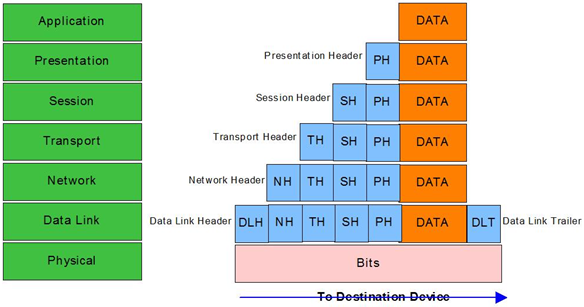
\includegraphics[width=\textwidth]{img/encapsulamiento}
	\caption{\small Encapsulamiento en el Modelo OSI, extra'ida de \cite{encapsulamiento}}
	\label{encapsulamiento}
\end{figure}

\vspace{1cm}

\item Establecimiento, control y cierre de la conexi'on.
\item Control de Flujo:
Asegurar que la velocidad de los datos no sature las posibilidades particulares de cada capa.
\item Control de Errores: Detecci'on y correcci'on de errores.
\item Multiplexaci'on: Posibilidad de compartir el canal entre varias conexiones.
\item Encriptaci'on y compresi'on.
\end{enumerate}

\section{TCP/IP}
\label{tcpip}
El conjunto de protocolos TCP/IP permite que computadoras de distintos tama'nos, marcas, y diferentes sistemas operativos puedan lograr una comunicaci'on entre s'i \citep{tcpipIluistrated}. Su desarrollo comenz'o hacia los a'nos 60', y en los 90' se convirtieron en los protocolos m'as utilizados en las redes.
Conforma la base de Internet, la \textsc{wan}\footnote{Wide Area Network, Red de 'Area Amplia} que conecta millones de dispositivos en todo el planeta.

Tiene un dise'no en capas similar al del Modelo OSI (ver Secci'on \ref{osi}), en donde cada capa provee una funcionalidad diferente para la comunicaci'on. El modelo posee 4 capas, Aplicaci'on, Transporte, Red y Enlace, como puede verse en la Figura \ref{tcpip}.

\begin{figure}[ht]
  	\centering
	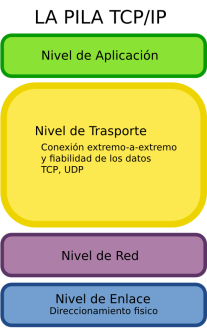
\includegraphics[width=140px]{img/tcpip}
	\caption{\small TCP/IP}
	\label{tcpip}
\end{figure}

\subsection{Las Capas}

\begin{enumerate}
\item Aplicaci'on

En esta capa se manejan los detalles de una aplicaci'on particular. Aqu'i se encuentran protocolos muy conocidos tales como HTTP (Hipertext Transfer Protocol), HTTPS (Hipertext Transfer Protocol Secure),  FTP (File Transfer Protocol), POP (Post Office Protocol), SMTP (Simple Mail Transfer Protocol), SNMP (Simple Network Management Protocol), Telnet (para login remoto), DNS (Domain Name System) \citep{redesComputadores}.
\clearpage
\item Transporte

Provee el servicio de env'io de flujo de datos entre dos hosts. En esta capa se encuentran 2 protocolos muy importantes:

	\subitem \textbf{TCP (Transfer Control Protocol):}
	\label{tcp}
	
	Permite crear conexiones entre hosts para el env'io de flujos de datos. Se ocupa de dividir los datos que vienen de la capa de aplicaci'on en paquetes de un tama'no adecuado para realizar el env'io en las capas inferiores. Tambi'en se encarga del control de la recepci'on de los paquetes enviados, as'i tambi'en como el establecimiento de los tiempos de espera para asegurarse que el otro extremo reconoce los paquetes enviados. Realiza la multiplexaci'on de la conexi'on, es decir, que permite compartir el canal entre varias conexiones.
	
	Para establecer la conexi'on entre los 2 extremos, el servidor debe dejar en ''escucha'' una direcci'on en un puerto determinado. El cliente, env'ia un mensaje SYN\footnote{SYNchronize.} inicial al servidor para iniciar la negociaci'on, el servidor contesta con un paquete SYN-ACK\footnote{ACKnowledgement.} que es contestado por el cliente por un ACK. Una vez intercambiados estos 3 mensajes, el cliente puede empezar a realizar las peticiones al servidor. Esto se llama Three Way Handshake (Negociaci'on de 3 v'ias), y puede verse en la Figura \ref{threeway}.
	
	\begin{figure}[ht]
  	\centering
	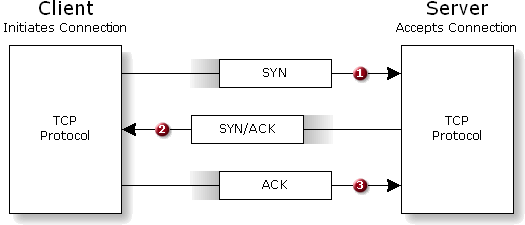
\includegraphics[width=380px]{img/threeway}
	\caption{\small Three Way Handshake, extra'ido de https://www.grc.com/}
	\label{threeway}
	\end{figure}

	\subitem \textbf{UDP (User Datagram Protocol):}
	
	Se ocupa de enviar paquetes de datos llamados datagramas de un extremo a otro, sin realizar una conexi'on previa, el mismo datagrama posee suficiente informaci'on para llegar a destino. No brinda ninguna garant'ia de que el paquete llegue a su destino y tampoco hace control de flujo.
\item Red

Esta capa, a veces llamada capa de Internet, maneja el movimiento de los paquetes a trav'es de la red. El enrutamiento y encaminamiento de los paquetes tiene lugar en esta capa. El protocolo principal de esta capa es IP (Internet Protocol), define el direccionamiento de la capa de red, los campos del datagrama, y las acciones tomadas por los routers y los sistemas finales sobre el datagrama bas'andose en los valores de dichos campos \citep{redesComputadores}. Otros protocolos de esta capa son: ICMP (Internet Control Message Protocol) e IGMP (Internet Group Management Protocol).

\item Enlace

Esta capa, a veces llamada capa de enlace de datos o capa de interfaz de red, incluye el driver\footnote{Controlador de Dispositivo} del sistema operativo y la correspondiente placa de red del dispositivo. Juntos se encargan de todos los detalles del hardware y de la interconexi'on f'isica con el medio (Cable, WiFi, Fibra 'Optica, etc.).
\end{enumerate}

\subsection{TCP/IP y el Modelo OSI}

Similitudes
\begin{enumerate}
\item Ambos se dividen en capas.
\item Ambos tienen Capa de Aplicaci'on, pero ofrecen servicios diferentes.
\item La capa de transporte y la de red son similares.
\item La conmutaci'on es por paquetes\footnote{M'etodo de env'io de datos, cada paquete posee datos e informaci'on de control que indica la ruta a destino.} (no por circuitos).
\end{enumerate}

Diferencias:
\begin{enumerate}
\item En la capa de aplicaci'on de TCP/IP se combinan las capas de presentaci'on y de sesi'on del Modelo OSI.
\item En la capa de enlace de TCP/IP se combinan las capas de enlace y de f'isica del Modelo OSI.
\item Al tener menos capas, TCP/IP es m'as simple.
\item TCP/IP es el est'andar de Internet, las redes no se desarrollan a partir del Modelo OSI, se utiliza como gu'ia.
\end{enumerate}

\begin{figure}[h]
  	\centering
	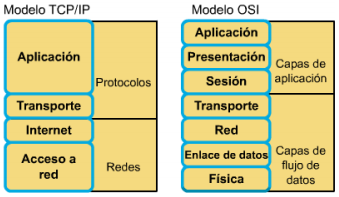
\includegraphics{img/tcpiposi}
	\caption{\small Comparaci'on entre TCP/IP y OSI}
	\label{tcpiposi}
\end{figure}

\clearpage

\section{HTTP}
\label{http}
Las siglas de este protocolo son por HyperText Transfer Protocol (Protocolo de Transferencia de Hipertexto). Es un protocolo de capa de aplicaci'on (ver Secci'on \ref{osi}) que sirve para distribuir informaci'on. Fu'e utilizado en la web desde el a'no 1990 en su primera versi'on (0.9), en la que simplemente se pod'ia transferir texto plano. Su evoluci'on fue el est'andar 1.0 en el que se mejor'o el protocolo permitiendo que los mensajes usen el formato \gls{mime}, se incorporaron metadatos acerca de la informaci'on transferida y modificadores en la sem'antica de petici'on/respuesta. La revisi'on del protocolo que se usa actualmente es la 1.1, definida en la RFC 2616 \citep{rfcHTTP1.1}. Contiene nuevos metodos, headers y otras caracter'isticas. Las principales diferencias de esta 'ultima definici'on se pueden ver en \citep{http1011}.

El contenido web reside en servidores, estos son los que se comunican utilizando este protocolo entre otros. Sirven \textsc{recursos}, estos recursos pueden ser p'aginas HTML, im'agenes, PDF's, video, etc, tanto contenido est'atico como din'amico (generado a demanda). Debido a la gran diversidad de contenido que provee un Servidor, es necesario identificar el tipo de recurso que se est'a enviando. Esto se hace utilizando una etiqueta llamada MIME-Type, que define el tipo de contenido a transferir.

Cada recurso del servidor tiene un nombre, para que los clientes puedan apuntar directamente al recurso deseado. Se nombra con una URL, que tiene el siguiente formato:

\begin{quote}
PROTOCOLO://SERVIDOR/PATH\_AL\_RECURSO/RECURSO
\end{quote}

El funcionamiento b'asico es, el cliente env'ia una petici'on al servidor (al puerto 80 por defecto) y este le responde. Esta comunicaci'on se realiza a trav'es de mensajes HTTP. Existen diferentes m'etodos que se pueden utilizar cuando se env'ia una petici'on al servidor, tales como

\begin{enumerate}
\item GET - El cliente solicita un recurso espec'ifico del servidor.
\item POST - El cliente env'ia datos que van a ser utilizados por el servidor.
\item HEAD - El cliente solicita s'olo los Headers (se detallar'an m'as adelante).
\end{enumerate}

Estos son algunos de los m'etodos, hay otros tales como PUT, DELETE, etc. Seg'un el m'etodo, el servidor opera de manera diferente. En la petici'on se env'ia el m'etodo, el recurso solicitado, la versi'on del protocolo utilizado, el host, el user-agent\footnote{Qui'en est'a generando la petici'on, por ejemplo Mozilla, Safari, Squid (browser, proxy, etc.).}, entre otros.
El servidor, responde a la petici'on con una respuesta, que contiene un c'odigo de estado de 3 d'igitos que le dice al cliente que la petici'on fue exitosa u otras, por ejemplo 200 (OK) o 404 (Documento no encontrado) de los m'as comunes.

Los mensajes de HTTP consisten en peticiones y respuestas, sus formatos son similares. Consisten en 3 partes:

\begin{enumerate}
\item Linea Inicial - Se indica que hacer en la petici'on o que fue lo que pas'o en la respuesta.
\item Headers - Ac'a se pueden definir diferentes par'ametros por c'ada l'inea con la sintaxis ''nombre:valor''.
\item Cuerpo - Esta parte contiene los datos enviados, ya sea del cliente al servidor o viceversa.
\end{enumerate}

El formato de una petici'on es el siguiente:

\begin{quote}
$<$m'etodo$>$ $<$url del recurso$>$ $<$versi'on$>$

$<$headers$>$

$<$cuerpo$>$
\end{quote}

El formato de la respuesta es el siguiente:

\begin{quote}
$<$versi'on$>$ $<$estado$>$ $<$descripci'on del estado$>$

$<$headers$>$

$<$cuerpo$>$
\end{quote}

\subsection{HEADERS}
\label{headers}
Los headers, a'naden informacion adicional a las peticiones y respuestas. El protocolo define varios headers, pero se pueden inventar tambi'en, los servidores y clientes son libres de hacerlo. Hay diferentes tipos de headers, entre los que se encuentran:

\begin{enumerate}
\item Headers generales

Pueden aparecer en peticiones y respuestas.
\item Headers de peticiones.

Proveen m'as informaci'on acerca de las peticiones.
\item Headers de respuesta.

Proveen informaci'on acerca del recurso del mensaje.
\item Headers de extensi'on

Permite agregar nuevos headers que no est'en dentro de la especificaci'on est'andar \citep{rfcHTTP1.1}.
\end{enumerate}

La definici'on completa de los headers se encuentra en la Secci'on 14 de \citep{rfcHTTP1.1}.

\section{HTTPS}

Los usuarios de Internet, utilizan la web para hacer transacciones que requieren que el nivel de seguridad sea fuerte. Operaciones como realizar transacciones bancarias o hacer compras online, no se realizar'ian si los datos que el usuario env'ia al servidor viajan desprotegidos. Ante esta necesidad, se combina el protocolo HTTP con la tecnolog'ia de encriptaci'on digital.
HTTPS es la versi'on ''segura'' de HTTP, a'nade a este protocolo, una capa de cifrado utilizando SSL \footnote{Secure Sockets Layer.} (el predecesor de TLS\footnote{Transport Layer Security.}) sobre TCP, como se puede ver en la Figura \ref{httpvshttps}. Se define en la RFC 2818 \citep{rfcHTTPS}. Se distingue el tr'afico seguro del inseguro por la utilizaci'on de un n'umero de puerto diferente.

\begin{figure}[h]
  	\centering
	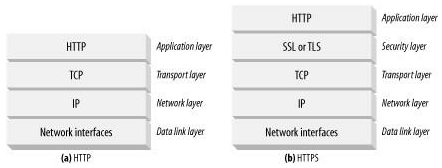
\includegraphics{img/httpvshttps}
	\caption{\small Comparaci'on entre HTTP y HTTPS, extra'ido de \citep{httpGuide}}
	\label{httpvshttps}
\end{figure}

Permite que los datos que viajan entre cliente y servidor vayan encriptados, esto se hace antes de enviar los datos por la red. Se distingue f'acilmente porque el formato de la URL empieza con https:// y la conexi'on por defecto se establece con el puerto 443. Es decir, si el browser hace una petici'on a un servidor, en la cual, el esquema es https, se inicia la negociaci'on para establecer la conexi'on segura con el mismo.

La conexi'on se hace con otro puerto diferente al de HTTP ya que SSL es un protocolo binario, completamente diferente. Si ambos llegaran al mismo puerto, los servidores interpretarian SSL como HTTP err'oneo y cerrar'ian la conexi'on.

\subsection{Criptograf'ia}

La criptograf'ia es el arte y la ciencia de codificar y decodificar mensajes, alterando la representaci'on lingu'istica de mensajes, buscando la confidencialidad y para prevenir la manipulaci'on de los mismos. Tambi'en se utiliza para probar quien fue el autor del mensaje o una transacci'on (no repudio).

Se basa en Algoritmos de Cifrado (Ciphers) que tienen un m'etodo para codificar el mensaje y otro para decodificarlo posteriormente. Comenzaron siendo algoritmos simples hasta que se empezaron a construir m'aquinas\footnote{Ver M'aquina Enigma Alemana, http://www.bbc.co.uk/history/topics/enigma} para reforzar la seguridad de la encriptaci'on haciendo operaciones m'as complejas. A causa de que estos algoritmos y m'aquinas pod'ian llegar a manos no apropiadas, se incluyeron diversos m'etodos (llaves met'alicas, diales de configuraci'on), que actuan como entrada para que el algoritmo o m'aquina pudiera funcionar. De esta manera, a'un teniendo el algoritmo o dispositivo, sin la clave no se puede decodificar.

En la era digital, los m'etodos (clave) para la entrada de los algoritmos de encriptaci'on son simplemente n'umeros. Estos algoritmos son funciones que toman una porci'on de datos y la codifican/decodifican basados en el algoritmo de encriptaci'on y la clave proporcionada.

\subsubsection{Criptograf'ia Sim'etrica}

La criptograf'ia puede ser sim'etrica, es decir, que la clave para encriptar y desencriptar el mensaje es la misma. De esta manera, tanto el emisor como el receptor deben intercambiarse previamente la clave, antes de comenzar la comunicaci'on.

El algoritmo m'as conocido de criptograf'ia sim'etrica es el DES (Data Encryption Standard) \citep{des}. Se trata de un algoritmo que utiliza claves de 56 bits para cifrar/descifrar bloques de datos de 64 bits. El uso de m'ultiples claves conduce al algoritmo Triple-DES, en el que DES se aplica 3 veces, consiste en 3 claves de 56 bits que se utilizan sucesivamente en los datos a cifrar/descifrar como puede verse en la Figura \ref{tripleDes}.

\begin{figure}[h]
  	\centering
	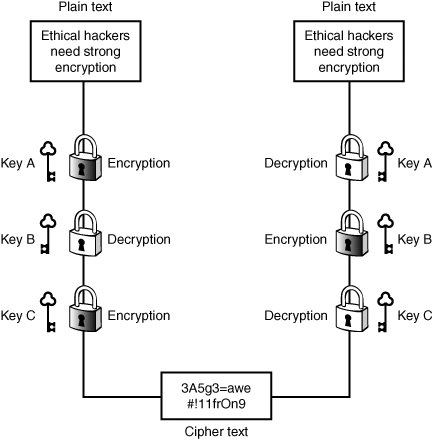
\includegraphics[width=200px]{img/tripleDes}
	\caption{\small Algoritmo Triple-DES, extra'ido de http://flylib.com/}
	\label{tripleDes}
\end{figure}

\subsubsection{Criptograf'ia As'imetrica}

En la criptograf'ia de clave p'ublica (ver Figura \ref{clavePublica}), las claves son Asim'etricas, es decir, que la clave para encriptar difiere de la clave para desencriptar el mensaje. En este tipo de criptograf'ia, la clave para encriptar el mensaje es p'ublica, cualquiera que quiera establecer una conexi'on con seguridad, puede obtener la clave\footnote{Almacenada en servidores de acceso p'ublico.} para iniciar la comunicaci'on. Por otro lado, la clave para desencriptar los mensajes es privada, pertenece al servidor que es el 'unico que puede decodificar los mensajes recibidos por el cliente.

\begin{figure}[h]
  	\centering
	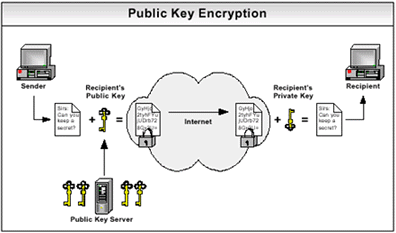
\includegraphics[width=300px]{img/clavePublica}
	\caption{\small Criptograf'ia de Clave P'ublica, extra'ido de http://www.novell.com/}
	\label{clavePublica}
\end{figure}

RSA (Rivest, Shamir y Adleman) \citep{rsa} es un algoritmo asim'etrico que se utiliza en firma digital\footnote{Mecanismo criptogr'afico que permite al receptor del mensaje poder determinar la entidad del emisor y confirmar que el mensaje no ha sido alterado desde que fue firmado.}. La clave utilizada para cifrar es diferente (pero relacionada) a la que se utiliza para descifrar. El algoritmo consta de los siguientes pasos:

\begin{enumerate}
\item Se seleccionan 2 n'umeros primos \textit{p} y \textit{q}.
\item Se calcula el producto de ambos n'umeros \textit{n = p * q}, este n'umero se llama \textit{m'odulo}.
\item Se elige un n'umero entero \textit{e} tal que \textit{1 $<$ e $<$ (p-1)*(q-1)}.
\item Se calcula \textit{d = $e^{-1}$ mod[(p-1)*(q-1)]}.
\end{enumerate}
La clave p'ublica es el par de n'umeros (n,e) y la clave privada es el par de n'umeros (n,d).

Para encriptar un mensaje \textit{m} se calcula:
\begin{quote}
$c \equiv m^e \pmod{n}$
\end{quote}
Para desencriptar un mensaje \textit{c} se calcula:
\begin{quote}
$\equiv c^d \pmod{n}$
\end{quote}

\subsection{Conexi'on}

Una conexi'on es el enlace que se establece entre el emisor y el receptor a trav'es del cual, se env'ia un mensaje. El procedimiento para iniciar una comunicaci'on HTTPS es el siguiente: El cliente abre una conexi'on con el puerto 443 al servidor. Una vez que la conexi'on TCP est'a establecida, el cliente y el servidor inicializan la capa SSL negociando algunos par'ametros criptogr'aficos e intercambiando llaves. Una vez concluida esta negociaci'on, ya pueden empezar a intercambiar mensajes encriptados. Se puede ver en detalle en la Figura \ref{httpsConnection}.

\begin{figure}[h!]
  	\centering
	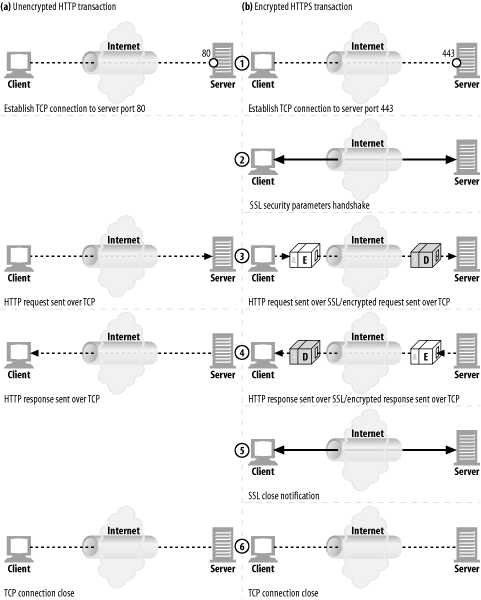
\includegraphics[width=390px]{img/httpsConnection}
	\caption{\small Establecimiento de Conexiones HTTP y HTTPS, extra'ido de \citep{httpGuide}}
	\label{httpsConnection}
\end{figure}